\documentclass[sigconf]{acmart}

\usepackage{booktabs} % For formal tables
\usepackage{multicol}
\graphicspath{{./figs/}}

% Dejavu fonts have unicode character support
% \usepackage{DejaVuSansMono}
\usepackage[T1]{fontenc}
\usepackage{lmodern}
\usepackage{listings}

\usepackage{ucs}
\usepackage[utf8x]{inputenc}
\usepackage{autofe}

% Copyright
%\setcopyright{none}
%\setcopyright{acmcopyright}
%\setcopyright{acmlicensed}
%\settopmatter{printacmref=false}
\setcopyright{rightsretained}
%\setcopyright{usgov}
%\setcopyright{usgovmixed}
%\setcopyright{cagov}
%\setcopyright{cagovmixed}

% DOI
\acmDOI{10.475/123_4}

% ISBN
\acmISBN{123-4567-24-567/08/06}

%Conference
\acmConference[LLVM in HPC'17]{LLVM in HPC: Fourth Workshop on the LLVM Compiler Infrastructure in HPC}{November 2017}{Denver Colorado, USA} 
\acmYear{2017}
\copyrightyear{2017}

%\acmPrice{15.00}

\begin{document}

\title{OpenMPIR}
\subtitle{Implementing OpenMP tasks with Tapir}
\author{George Stelle}
\affiliation{\institution{Los Alamos National Laboratory}}
\email{stelleg@lanl.gov}

\author{Stephen Olivier}
\affiliation{\institution{Center for Computing Research \\ Sandia National Laboratories}}
\email{slolivi@sandia.gov}

\author{Pat McCormick}
\affiliation{\institution{Los Alamos National Laboratory}}
\email{pat@lanl.gov}

\begin{abstract}
Optimizing compilers for task-level parallelism are still in their infancy.
This work implements a frontend which compiles a subset of OpenMP tasks to
Tapir IR. This enables analyses and optimizations previously inaccessible to
OpenMP codes. Initial performance results for the Barcelona OpenMP tasking
suite and show performance improvements over existing OpenMP compiler
implementations. 
\end{abstract}

\maketitle

\section{Introduction}

When writing task-parallel programs today, one has a large selection of
programming models. Unfortunately, despite having significant overlap in
semantics, parallel programming models like OpenMP, Cilk, Kokkos, HPX, Charm++,
Qthreads, pthreads, MPI, Chapel, UPC, etc. have virtually no ability to
interoperate, both at compile time and run time. In addition, many of these
programming models are implemented as libraries, and therefore have no compiler
support. There has been some recent work on specializing compilers to reason
about libraries \cite{kokkos}, but the fragmentation among the models that
presents another challenge for compiler writers, which must choose a single
model to analyze and optimize. An ideal solution would be some some form of
common representation of parallelism that all IRs can share.

Internal representations (IRs) are the compiler objects on which almost all
analyses and optimizations are performed. Historically, a major drawback for
parallel codes is that IRs don't have the ability to represent, and therefore
reason about, parallelism. This prevents the application of common
optimizations to concurrent code. The recent work of Schardl et al.
\cite{shardl2017} has shown that standard compiler IRs can be extended to
represent fork-join parallelism. In that work, by extending the LLVM
instruction set with three instructions, they are able to capture all of the
semantics to implement the semantics of Cilk, an extension to C. They suggested
that a similar approach could be taken with OpenMP tasks.

In this work, we put that suggestion to the test, implementing OpenMP tasks by
compiling them to Tapir instructions. This enables us to target non-openmp
runtimes and compare performance to existing OpenMP implementations. Specifically,
we run our prototype implementation on the Barcelona OpenMP task suite
\cite{barcelona}. We discuss the kinds of optimizations this enables, and how
the work could be extended to include other parallelism constructs and semantics
in OpenMP. We also discuss the possibility of extending this work to other
programming models, which would help to alleviate some of the fragmentation
issues discussed above.

The contributions of this work include: 

\begin{itemize}
\item A prototype frontend from OpenMP task constructs to Tapir IR
\item Benchmarks of the implementation, showing performance improvements over
existing OpenMP implementations
\item An initial investigation into the reasons for the performance improvement
\end{itemize}

Our hope for this paper is that it moves the community towards a shared IR that
can be used for many programming models. This work presented in this paper only
represents a small step in that direction, and there is still a herculean amount
of work required. We argue that the benefits vastly outweigh the costs, and
hope to see more work follow suite. 

\subsection{Outline}

The remainder of the paper is organized as follows: In Section~\ref{Sec:background} 
we give background and motivation for the paper. Following that, we describe OpenMP
tasking in Section~\ref{Sec:OpenMP}, and Tapir in Section~\ref{Sec:Tapir}. We then 
discuss the implementation, and how we compile OpenMP task constructs to Tapir IR in
Section~\ref{Sec:Implementation}. In Section~\ref{Sec:Evaluation} we describe the 
evaluation setup, including what implementations we compare to and how. We discuss
the results of evaluation in Section~\ref{Sec:Results}, including possible
explanations for discrepancies. Finally, we discuss how the many ways the work can
be extended in Section~\ref{Sec:Future}, and conclude in Section~\ref{Sec:Conclusion}.

\section{Background} \label{Sec:Background}

Internal representations are a crucial part of modern compilers. By representing
code in a generic, hardware-agnostic format, they allow both multiple frontends for
different source languages, and multiple backends for different hardware, to all
take advantage of a series of compiler optimizations and analyses. 

LLVM is arguably the most successful IR to date \cite{llvm}. By implementing a simple
single static assignment (SSA) representation, it enables powerful optimizations 
that are effective for a wide range of programming languages and hardware
\cite{llvm imps}. 

Historically, LLVM has had a sequential semantics: there is no notion of
concurrent or parallel processes. This resulted in existing compilers treating 
parallelism constructs as thin wrappers for calls into runtime systems. These
calls are essentially impossible for the compiler to reason about, due to the
complexity of runtimes being called. 

This unfortunate situation was recently remedied by Schardl et al.
\cite{tapir}. By adding three instructions to LLVM, Tapir enables analyses and
optimizations of parallel code. A full description 

\subsection{Fragmentation}

In this section we discuss a significant challenge in HPC: fragmentation of
parallel programming models. There are many, many, many ways to write
parallel programs \cite{....}. From libraries, to language extensions, to
standalone languages, to combinations of the above, it can be hard to choose
the right one. This means that when writing tooling, optimizations, or
analyses, one has to choose which model to target. One common difficulty among
all of these is that reasoning about parallel programs is hard \cite{}, and
compilers can help \cite{}. Therefore any duplicated work is extremely costly.
This is exactly analogous the problem LLVM helps to solve. Many optimizations
and analyses can be applied across a wide range of programming languages and 
hardware, but until there was an effective IR, those were often duplicated, 
resulting in a lot of lost opportunity. 

Addressing these concerns this is a major motivation for our turning to Tapir.
By standardising a powerful but simple internal representation and building
frontends and backends for it, one both make it easier to build optimizations
and analyses for a given programming model, and avoid duplicating that work
across different implementations. We'll return to this issue later in the paper
when discussing potential limitations and challenges for Tapir for other
hardware and 

\section{Tapir} \label{Sec:Tapir}

\section{OpenMP Tasks} \label{Sec:OpenMP}

Initially, the cross-vendor OpenMP~\cite{spec} shared memory programming model 
focused on the execution of data parallelism by a cooperating team of threads, 
e.g., dividing the iterations of a loop among the threads. Version 3.0 of the 
OpenMP API specification introduced support for lightweight asynchronous tasks, 
designated by the application developer and scheduled onto the team of threads 
by the OpenMP run time implementation.  The \texttt{task} construct applied to 
a structured block of code creates an explicit task, and the \texttt{taskwait} 
construct waits for completion of all tasks generated by the current task.

Recursive task creations and synchronizations using the constructs result in 
an implicit directed acyclic graph (DAG) that allows both reasoning about and 
visualization of the program execution.  Figure~\ref{Fig:fib-graph-to-schedule}
shows some example code, a view of the task DAG, and a simplified execution 
schedule mapping the tasks to a team of two threads.  In the example, the Nth 
Fibonacci number is calculated by recursively generating tasks to calculate 
the (N-1)th and (N-2)th Fibonacci numbers.  The \texttt{taskwait} ensures that 
the child tasks have completed before their answers are combined to yield the 
final result.

\lstset{basicstyle=\tt\small, language=C, 
morekeywords={omp, for, pragma, omp, task, taskwait}}
\begin{figure*}
\begin{center}
\begin{tabular}{| c c c | c c c | c c c |}
\hline
 & 
\begin{lstlisting}
int fib(int n) 
{                    // A
  if (n < 2)
    return n;
  else
  {
    int x, y;
    #pragma omp task
      x = fib(n-1);  // B
    #pragma omp task
      y = fib(n-2);  // C
    #pragma omp taskwait
    return (x+y);    // D
  }
}
\end{lstlisting}
& & &
    \centering{
   \raisebox{-0.6in}{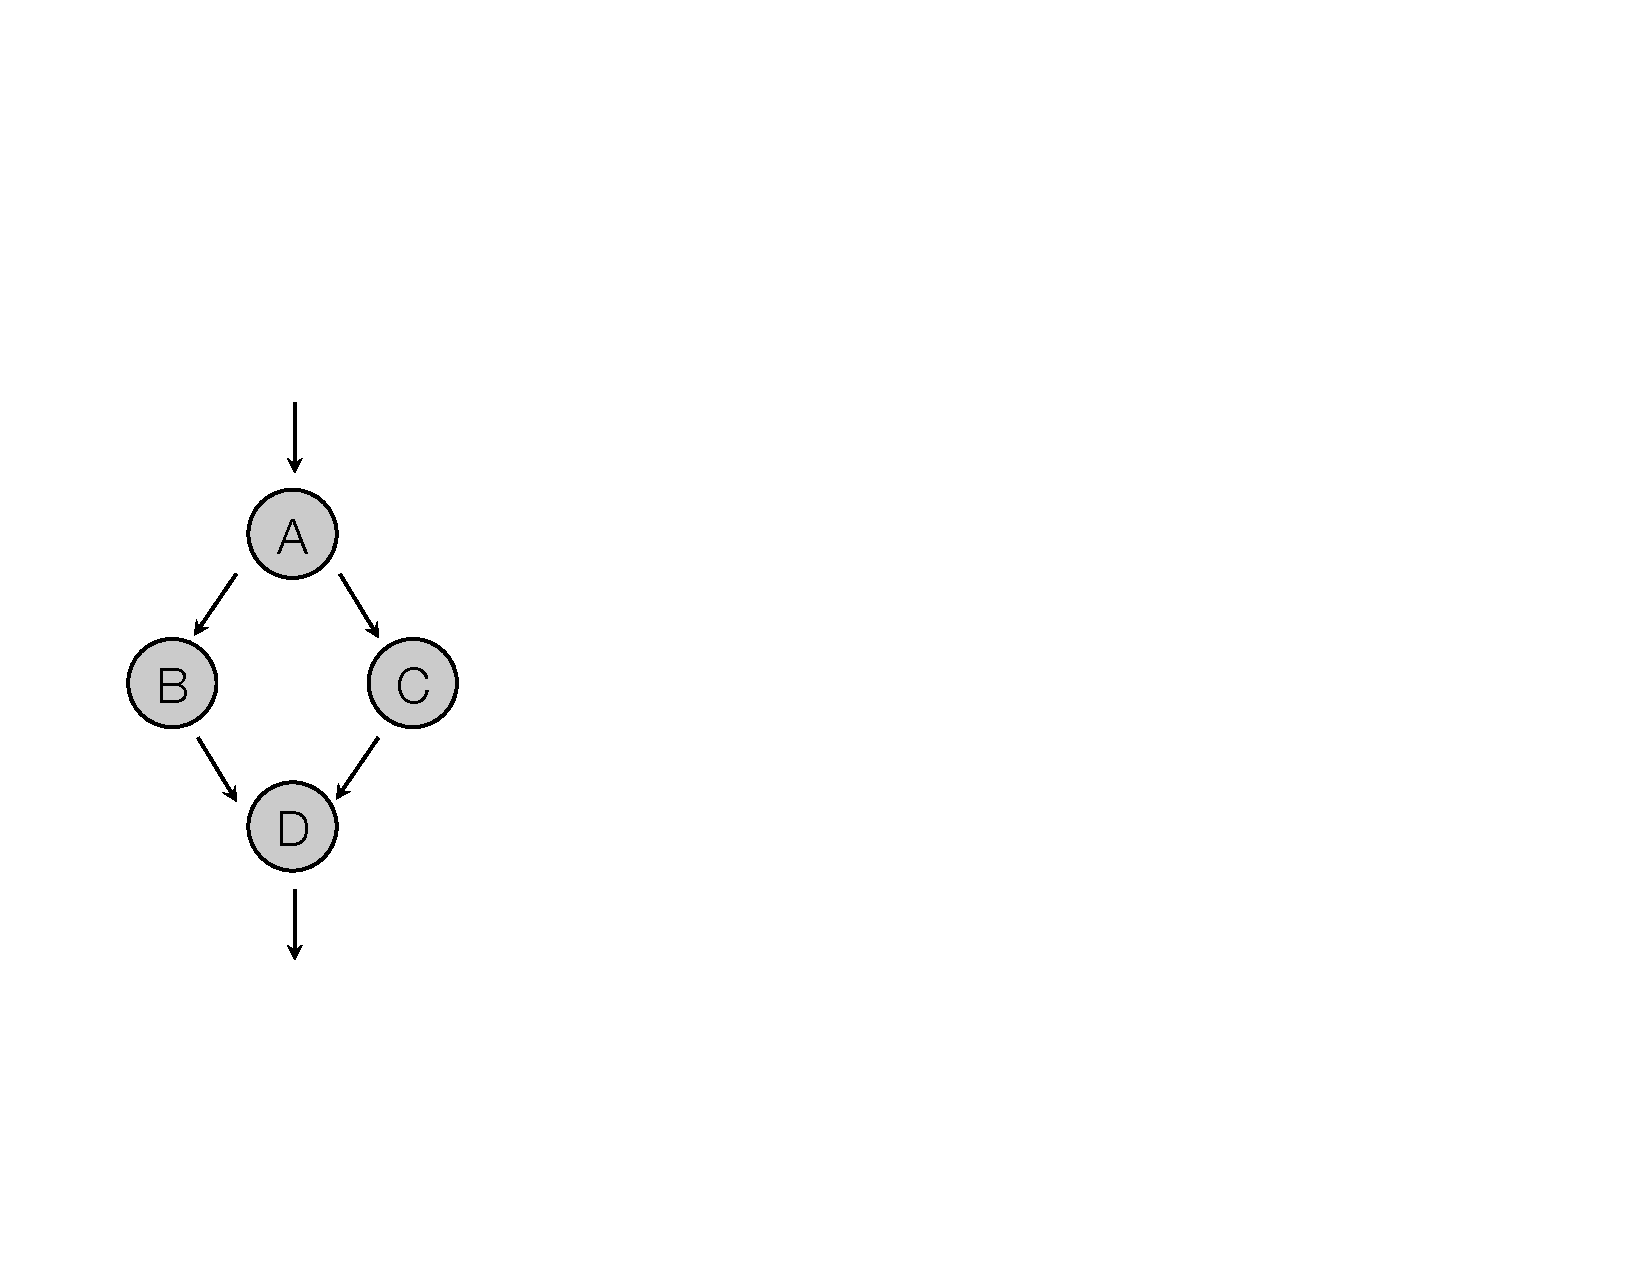
\includegraphics[scale=0.35]{fib-task-graph.pdf}}
    }
& & &
    \centering{
     \raisebox{-0.25in}{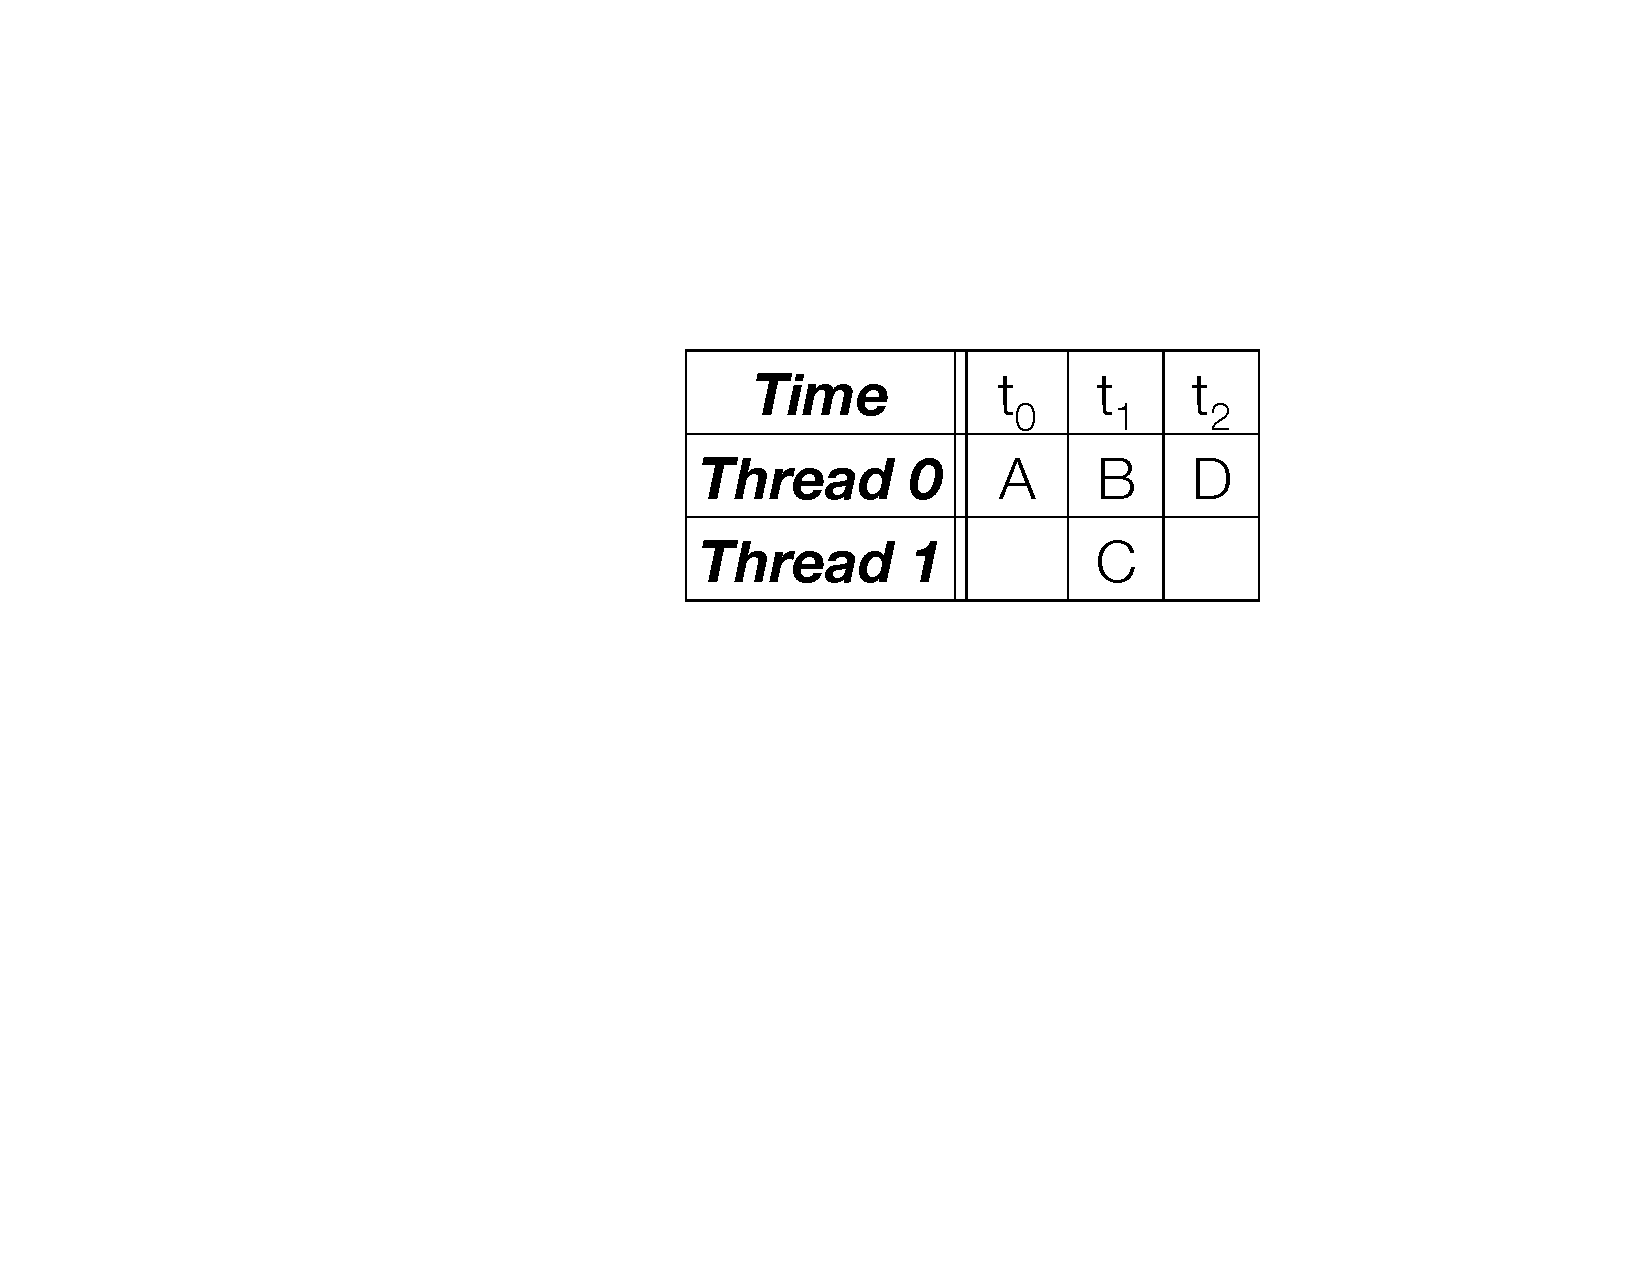
\includegraphics[scale=0.35]{fib-schedule.pdf}}
    }
 &  \\
\hline
\end{tabular}
\end{center}
\caption{Code, task graph, and schedule of a simple brute force recursive 
Fibonacci number calculation on two threads.}
\label{Fig:fib-graph-to-schedule}
\end{figure*}

The initial design of the OpenMP task model~\cite{ayguade09design} established 
a basic framework for asynchronous task parallel execution in OpenMP programs.
Subsequent versions of the OpenMP specification up to the current version 4.5 
have added additional new features to the tasking model.  The \texttt{depend} 
clause codifies data dependences among tasks, indicating that a data location 
is an input or output of a task.  The run time system ensures that a task is 
not scheduled until its input dependences are fulfilled.  The \texttt{taskloop} 
construct combines groups of independent loop iterations into explicit tasks, 
enabling composition of concurrent loop execution and independent explicit 
tasks within the same OpenMP parallel region. The \texttt{taskgroup} construct 
waits on not only all child tasks, but all descendent tasks, providing a deep 
synchronization. The \texttt{taskwait} construct allows the application to 
indicate a point at which the implementation may suspend the current task to 
work on other tasks, as may be desired for long-running tasks that generate 
many others.  The task concept was also leveraged to provide for asynchronous 
offload of data and computation to accelerators by applying the \texttt{nowait} 
clause to device constructs like the \texttt{target} construct to generate an 
asynchronous \textit{target task}.

Several clauses for the \texttt{task} construct aim to optimize execution of 
tasks but can be safely ignored by an implementation that chooses to do so. 
The \texttt{mergeable} clause allows the implementation to omit creation of a 
new data environment for a descendent of a task marked with the \texttt{final}
clause.  The \texttt{priority} clause assigns an integer priority to the task 
and recommends the prioritization of tasks with higher priority values.
The \texttt{untied} clause allows a task to be migrated between threads after 
suspension, which enables practical use of \textit{work-first scheduling} 
(suspending the parent task in favor of executing each child task immediately 
on the thread where it is generated).

\section{Implementation}

Tapir is implemented as an extension to the LLVM instruction set. Clang is a
C family compiler that has support for OpenMP extensions \cite{clang} and targets
LLVM. The existing Clang OpenMP implementation mapps OpenMP constructs directly
to OpenMP runtime library calls, by wrapping a C statement in a
\texttt{CapturedStmt}.  This replaces a C statement with a function call into
the OpenMP runtime library. along with a machine generated function who's body
contains that statement. 

For this work, we replaced a subset of the OpenMP implementation to generate
Tapir IR instead of vanilla LLVM IR with OpenMP runtime calls. Specifically, we
replace the two primary pragmas for task parallelism: \texttt{task\_spawn} and
\texttt{task\_wait}. By re-using code from Schardl et al. for code generation
of Cilk constructs, we were able to easily generate Tapir code for these OpenMP
pragmas. The ease with which this was completed is a testament to the quality of
the Tapir implementation. 

While we did implement the codegen for the \texttt{task\_spawn} and
\texttt{task\_wait} constructs, it's worth noting here that even for these
pragmas, the implementation is incomplete. Currently, any clauses modifying the 
behaviour of the pragmas is ignored. Probably the most common semantics this
will change of variable semantics, e.g. \texttt{shared} vs. \texttt{private}.
Surprisingly, this had little effect on the correctness of the entire Barcelona
OpenMP task suite. Indeed, it is likely that fixing this issue would increase
the performance of this work marginally, due to reducing the number of memory
copies for variables declared \texttt{private} in OpenMP code. 

The surprising fact that program behaviour wasn't changed significantly is
worth visiting here. We surmise that it is likely due to the variable semantics
borrowed from the Cilk codegen and their relation to the OpenMP specification
of semantics.  In particular, \emph{OpenMP doesn't specify any memory model for
shared variables}. This results in the Cilk style of only writing to a shared
variable at the end of a parallel section as a perfectly valid implementation
of OpenMP's specification. In contrast, existing OpenMP implementations often
write to shared variables on every write. This is a potential for performance
discrepancy due to differing implementation-defined behaviour, and we will 
return to it when discussing performance on the Barcelona OpenMP task suite.
There is of course the fact that technically, by copying the value of variables
back to the surrounding context even for \texttt{private} variables, one isn't
following the specification. We surmise that in practice this hasn't had an
effect due to the fact that \texttt{private} variables are generally used for
performance, rather than their semantic properties. 

A very important property to discuss of the current implementation is the
backend. This work has \emph{only been on the frontend}, which means we use
the only existing backend for Tapir. The existing backend is to generate 
calls into the Cilk runtime, \texttt{libcilkrts}. This obviously has many 
implications for adhering to the OpenMP specification. For example, environment
variables such as \texttt{OMP\_NUM\_THREADS} are ignored, replaced by
\texttt{CILK\_NWORKERS}. We discuss some of these issues below, and return to 
address others in the future work section. 

There are other issues that had to be overcome to run full OpenMP programs
using Tapir as described above. Generally, a program has to contain other
OpenMP pragmas in order to run parallel code. A standard pattern for building
task-parallel OpenMP programs is to start a \texttt{parallel} pragma to spin up
the necessary hardware threads, then have a \texttt{single} pragma to have only
one thread continue on the specified statement. Then the other threads will get
work from spawned tasks, instead of implicitly executing the same code in a
data parallel style. For the purpose of this paper, we took the shortcut of
replacing these pragmas with no-ops. This worked well for all examples except
for one, in which after the \texttt{parallel} and \texttt{single} pragmas the
top level task was called with an unnecessary \texttt{task} pragma. Because the
wait was implicit and unhandled by our implementation, the simple fix was to
remove the \texttt{task} pragma. This was the only change required to the 
source code. Our temporary no-op shortcut, of course, doesn't follow the OpenMP
specification, and should be addressed by future work. 

All code used for the implementation is available at \\
\texttt{https://github.com/lanl/openmpir}. The version used for this paper is
tagged as LLVM17.

\subsection{Example} \label{Sec:Example}

To better understand how the OpenMP to Tapir compiler works, we turn to the
\texttt{fib} example from Section~\ref{Sec:OpenMP}. In Figure~\ref{Fig:Example}
we show what Tapir code is generated.  

\begin{figure*}
\begin{tabular}{| c c c | c c c |}
\hline
 & 
\begin{lstlisting}
int fib(int n) 
{                    // A
  if (n < 2)
    return n;
  else
  {
    int x, y;
    #pragma omp task
      x = fib(n-1);  // B
    #pragma omp task
      y = fib(n-2);  // C
    #pragma omp taskwait
    return (x+y);    // D
  }
}
\end{lstlisting}
& & &
\begin{lstlisting}
if.end:                                 
  detach within %syncreg, label %det.achd, label %det.cont

det.achd:                                 
  %2 = load i32, i32* %n.addr, align 4
  %sub = sub nsw i32 %2, 1
  %call = call i32 @fib(i32 %sub)
  store i32 %call, i32* %x, align 4
  reattach within %syncreg, label %det.cont

det.cont:                                   
  detach within %syncreg, label %det.achd1, label %det.cont4

det.achd1:                                
  %3 = load i32, i32* %n.addr, align 4
  %sub2 = sub nsw i32 %3, 2
  %call3 = call i32 @fib(i32 %sub2)
  store i32 %call3, i32* %y, align 4
  reattach within %syncreg, label %det.cont4

det.cont4:                                  
  sync within %syncreg, label %sync.continue
\end{lstlisting}
 &  \\
\hline
\end{tabular}

\caption{Compilation to Tapir}
\label{Fig:Example}
\end{figure*}

\section{Evaluation} \label{Sec:Evaluation}

For evaluation we compared performance on the Barcelona OpenMP task suite to 
existing OpenMP implementations. The Barcelona OpenMP task suite is a set of 
tests intended to test performance of OpenMP implementations using both
irregular and regular tasking. The benchmarks are described in
Figure~\ref{Fig:benchmark_desc}. The benchmark suite has added an unbalanced
tree search benchmark since the paper was published.  Unfortunately, this seems
to be buggy, and failed on every implementation for even medium input sizes. We
have therefore left it out of our evaluation.

\begin{itemize}
\item \texttt{Alignment}: aligns all protein sequences from  an  input
file  against  every  other  sequence  using  the Myers  and Miller \cite{}
algorithm. The alignments are scored and the best score for each pair is
provided as a result. The scoring method is  a  full  dynamic  programming
algorithm. It uses  a  weight matrix to score mismatches, and assigns
penalties for opening and extending gaps. The output is the best score for each
pair of them.
\item \texttt{FFT}: computes the one-dimensional Fast Fourier Transform
of a vector of n complex values using the Cooley-Tukey \cite{cooley-tukey}
algorithm. This is a divide and conquer algorithm that  recursively  breaks
down a Discrete Fourier Transform (DFT) into many smaller DFT’s. In each of the
divisions multiple tasks are generated.
\item \texttt{Fibonacci}: computes the n'th fibonacci number using a  recursive
paralellization. While  not  representative  of  an efficient  fibonacci
computation  it  is  still  useful  because  it  is a simple test case of a
deep tree composed of very fine grain tasks.  
\item \texttt{Floorplan}: kernel computes the optimal floorplan distribution
of a number of cells. The algorithm gets an input file with  cell’s
description  and  it  returns  the  minimum  area  size which includes all
cells. This minimum area is found through a recursive branch and bound search.
We hierarchically generate tasks  for  each  branch  of  the  solution  space.
The  state  of  the algorithm needs to be copied into each newly created task
so they can proceed. This implies that additional synchronizations have been
introduced in the code to maintain the parent state alive.
\item \texttt{Health}: simulates de Columbian Health Care System \cite{?}. It
uses multilevel lists where each element in the structure  represents  a
village with  a  list  of  potential patients and one hospital. The hospital
has several double-linked lists representing the possible status of a patient
inside it (waiting, in assessment,   in   treatment   or   waiting   for
reallocation).  At  each time step  all  patients  are  simulated  according
with several probabilities (of getting sick, needing a convalescence treatment,
or  being  reallocated to  an  upper  level  hospital).  A  task  is  created
for  each  village being  simulated.  Once  the lower   levels   have   been
simulated synchronization   occurs. 
\item \texttt{NQueens}: computes  all  solutions  of  the n-queens
problem, whose objective is to find a placement for $n$ queens on an $n \;
\times \; n$ chessboard such that none of the queens attack any other. It uses
a backtracking search algorithm with pruning. A task is created for each step
of the solution.
\item \texttt{Sort}: sorts a random permutation of n 32-bit numbers with  a
fast  parallel  sorting  variation  \cite{mergesort}  of  the  ordinary
mergesort.  First, it divides an array of elements in two halves, sorting  each
half  recursively,  and  then  merging  the  sorted halves with a parallel
divide-and-conquer method rather than the  conventional  serial  merge.  Tasks
are  used  for  each  split and merge. When the array is too small, a serial
quicksort is used  so increase  the  task  granularity.  To  avoid  the
overhead of  quicksort,  an insertion  sort  is  used  for  very  small  arrays
(below a threshold of 20 elements).
\item \texttt{SparseLU}: computes an LU matrix factorization over
sparse matrices. A first level matrix is composed by pointers to  small
submatrices  that  may  not  be  allocated.  Due  to  the sparseness  of  the
matrix,  a  lot  of  imbalance  exists.  Matrix size and submatrix size can be
set at execution time. While a dynamic schedule can reduce the imbalance, a
solution with tasks parallelism seems to obtain better results \cite{}. In each
of the sparseLU  phases,  a  task  is  created  for  each  block  of  the
matrix that is not empty.
\item \texttt{Strassen}: algorithm  uses  hierarchical  decomposition of a
matrix for multiplication of large dense matrices \cite{}. Decomposition is
done by dividing each dimension of the matrix into  two  sections  of  equal
size. For each decomposition a task is created. 
\end{itemize}

There are two classes of input sizes for the benchmarks. Some, like Floorplan,
require input files. For each of these, we chose the largest provided. For the
benchmarks with a parameter to adjust the size of the input, we attempted to 
choose a parameter size so that the fastest implementation was on the order of
seconds. The exact inputs used are:

\begin{itemize}
\item \texttt{Alignment: -f prot.100.aa} 
\item \texttt{FFT: -n 335544320}
\item \texttt{Fibonacci: -n 48}
\item \texttt{Floorplan: -f input.20}
\item \texttt{Health: -f large.input}
\item \texttt{NQueens: -n 15}
\item \texttt{Sort -n 335544320}
\item \texttt{SparseLU: -n 100 -m 100}
\item \texttt{Strassen: -n 8192}
\end{itemize}

For other implementations, we compare to GCC 7.1, Clang 4.0.1, and Intel
17.0.0. The machine used is a two socket Intel Xeon E5-2693 v3 machine with
132GB of memory, running Linux 4.11.4. All benchmarks were run using all 64
hyper-threads. 32 thread tests were done as well and showed qualitatively
similar results. It's worth noting that each of the other implementations comes
with it's own runtime. In this sense, performance is a function of both the
compiler and any optimizations it's able to perform, and the runtime.
Understanding the interaction of these two parts is non-trivial, as we will see
when discussing results. 

As mentioned in the Section~\ref{Sec:Implementation}, the gaps in the implementation
changed program behaviour in a couple cases. In the case of \texttt{FFT}, we were
forced to remove an unecessary \texttt{task} pragma, as the current implementation
doesn't insert the implicit barrier at the end of a \texttt{parallel} region. This 
was a one line fix in the benchmark, and would be fixed properly by handling
the \texttt{parallel} and \texttt{single} pragmas correctly in our implementation. 

The second change in program behaviour due to our incomplete implementation was
caused by the lack \texttt{critical} pragma and \texttt{atomic} pragmas. This
issue showed up in the \texttt{Floorplan} benchmark. The \texttt{critical} pragma
ensures that only one thread can executed the referred statement at a time. 
This should be fixable in the implementation by adding a simple code-localized
synchronization generation in the IR. Similarly, the \texttt{atomic} pragma 
can be addressed by retaining a pointer to the shared stack variable, much like
existing OpenMP implementations. It is worth noting that this behaviour was
non-deterministic, and that roughly half of the time the Floorplan still
returned correct results. As we will see, this makes for an interesting
trade-off given the performance increase witnessed.

In our evaluation, we caught three kinds of errors:

\begin{itemize}
\item Segmentation faults
\item Timeouts (10 Minutes)
\item Non-determinism in result correctness
\end{itemize}

We set a timeout of 10 minutes, as at least one implementation was always
finishing within ~10 seconds, anything running more than 60 times slower
becomes irrelevant. Due to time constraints, correctness checks were not
performed on every run, so it is possible some non-determinism was missed. 

Each variant was run 10 times, with the height of the bars representing the
mean and the error bars representing standard deviation. In cases where there
was timeout or segmentation fault, no time is reported, and the run is marked
as faulty.

\section{Results} \label{Sec:Results}

In this section we discuss the results of running our evaluation on our
implementation, and how its performance compared to the existing
implementations listed in Section~\ref{Sec:Evaluation}. See
Figure~\ref{Fig:results} for a simple visualization of the performance. Each
graph represents a single benchmark from the previously enumerated Barcelona
benchmarks, and each bar represents one of the implementations. 

\begin{figure*}
\begin{multicols}{2}
  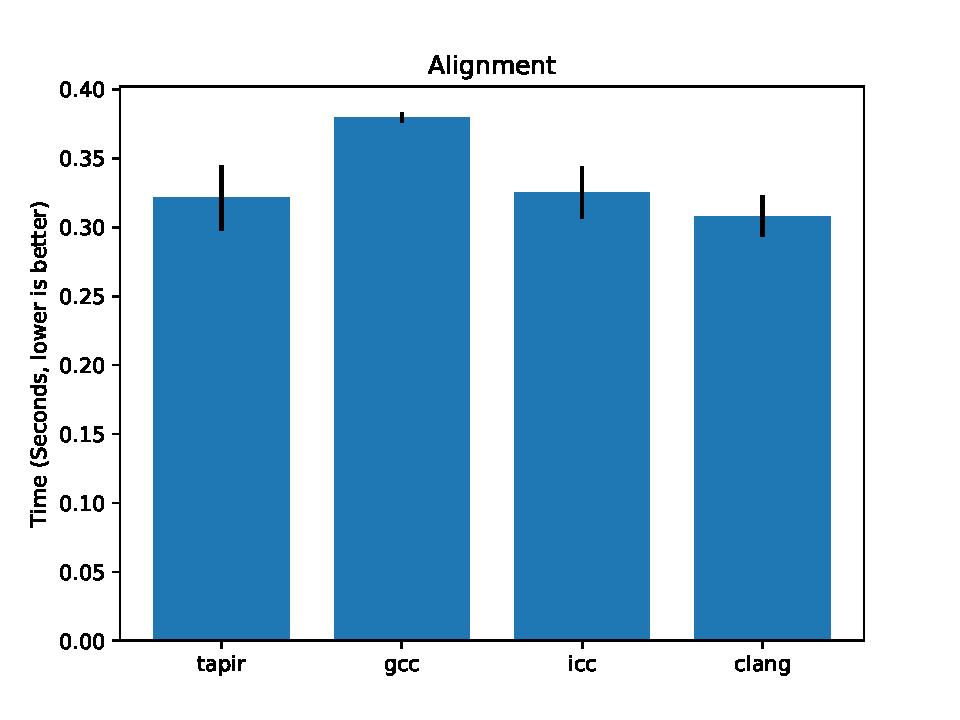
\includegraphics[width=\linewidth]{alignment.pdf} \par
  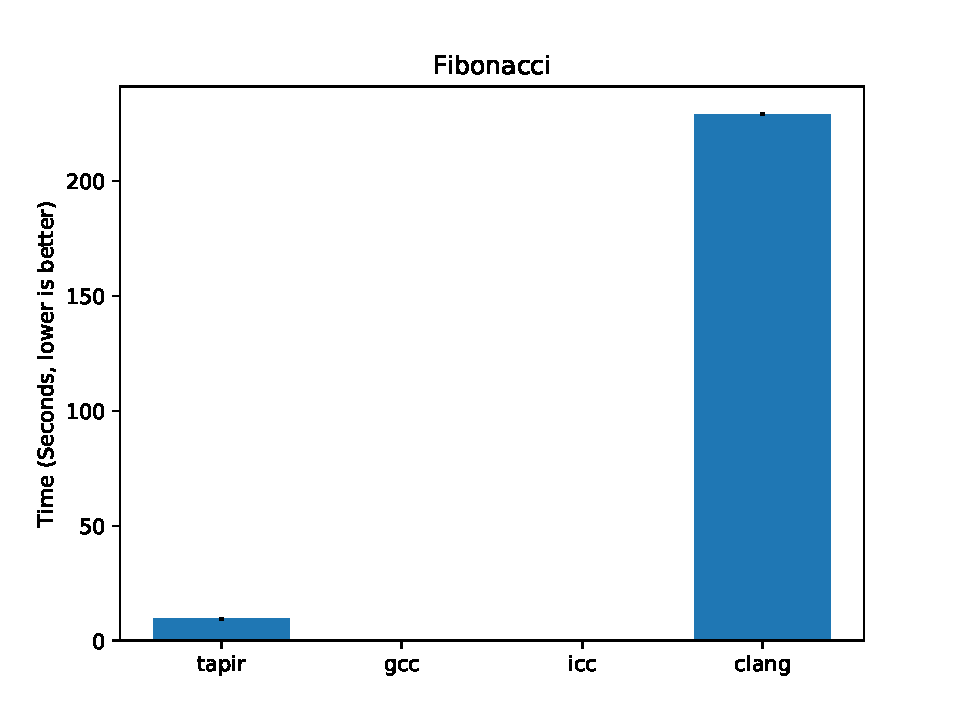
\includegraphics[width=\linewidth]{fib.pdf} 
  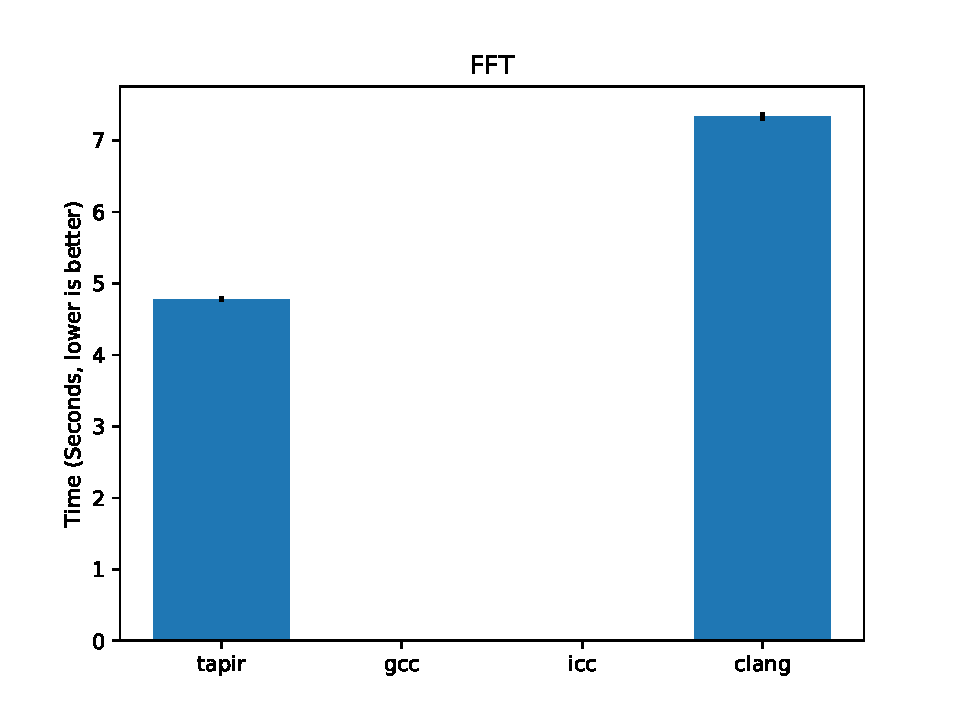
\includegraphics[width=\linewidth]{fft.pdf} \par
  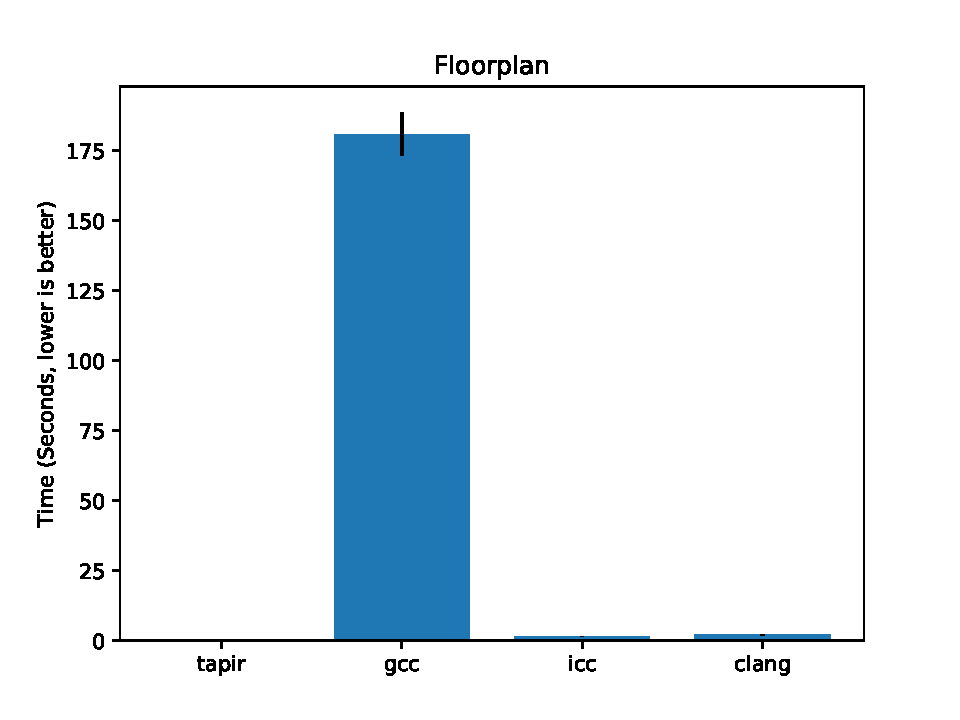
\includegraphics[width=\linewidth]{floorplan.pdf} 
  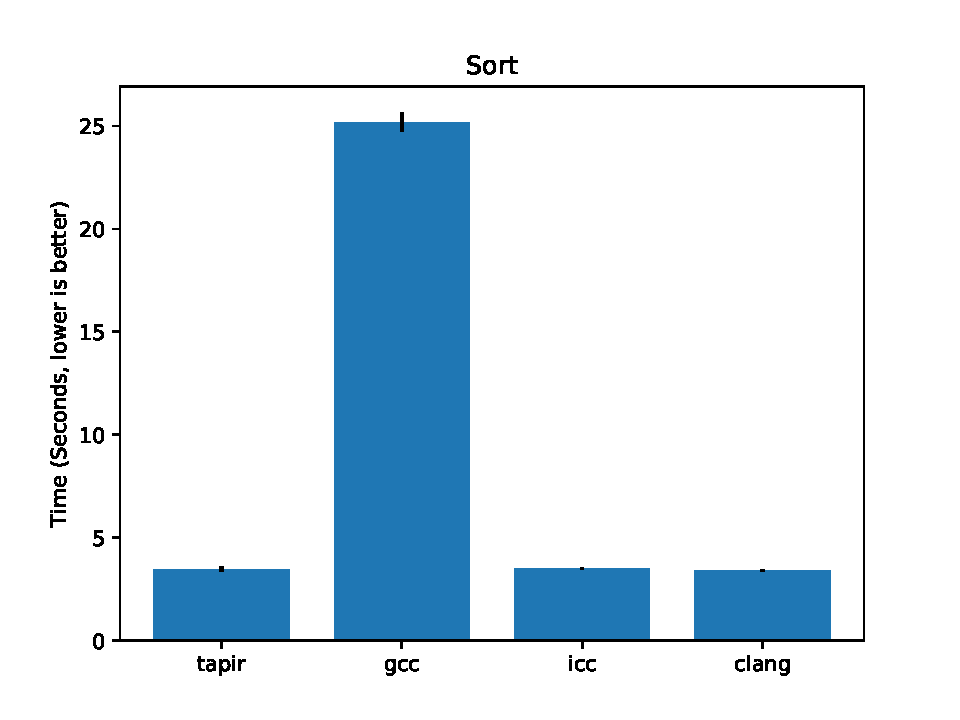
\includegraphics[width=\linewidth]{sort.pdf} \par
  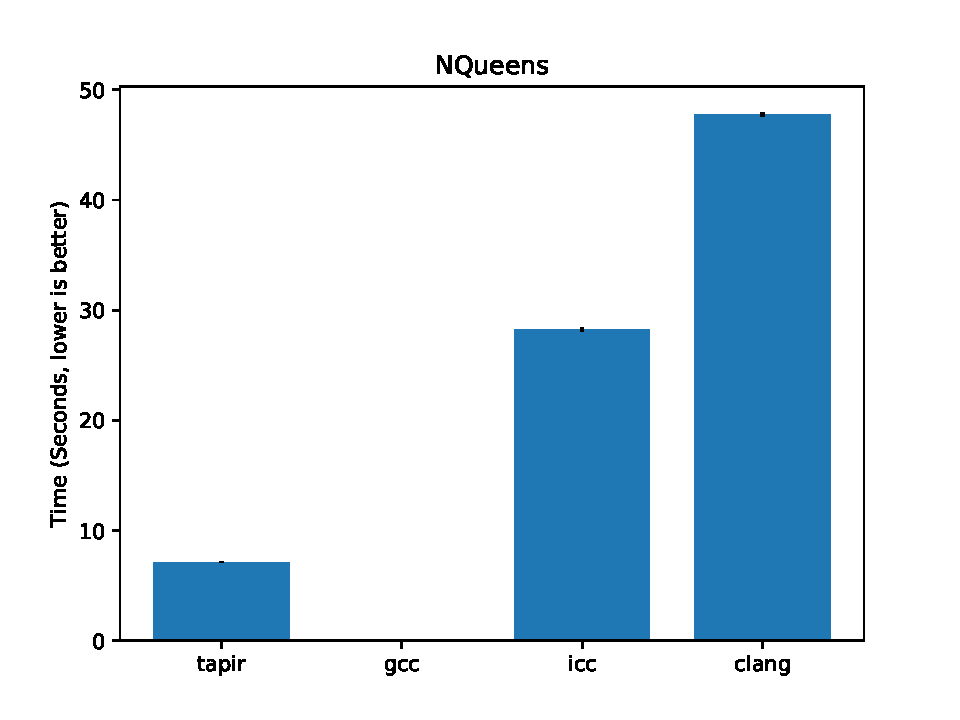
\includegraphics[width=\linewidth]{nqueens.pdf}
\end{multicols}
\caption{Barcelona OpenMP Task Suite Results}
\end{figure*}

\begin{figure*}
\begin{multicols}{2}
  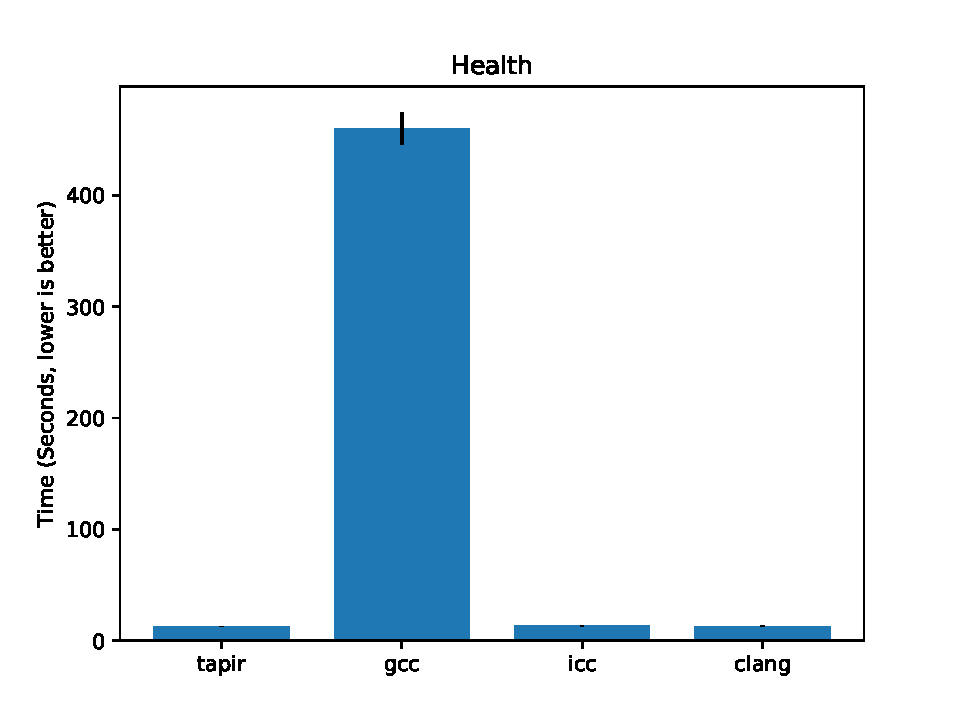
\includegraphics[width=\linewidth]{health.pdf} \par
  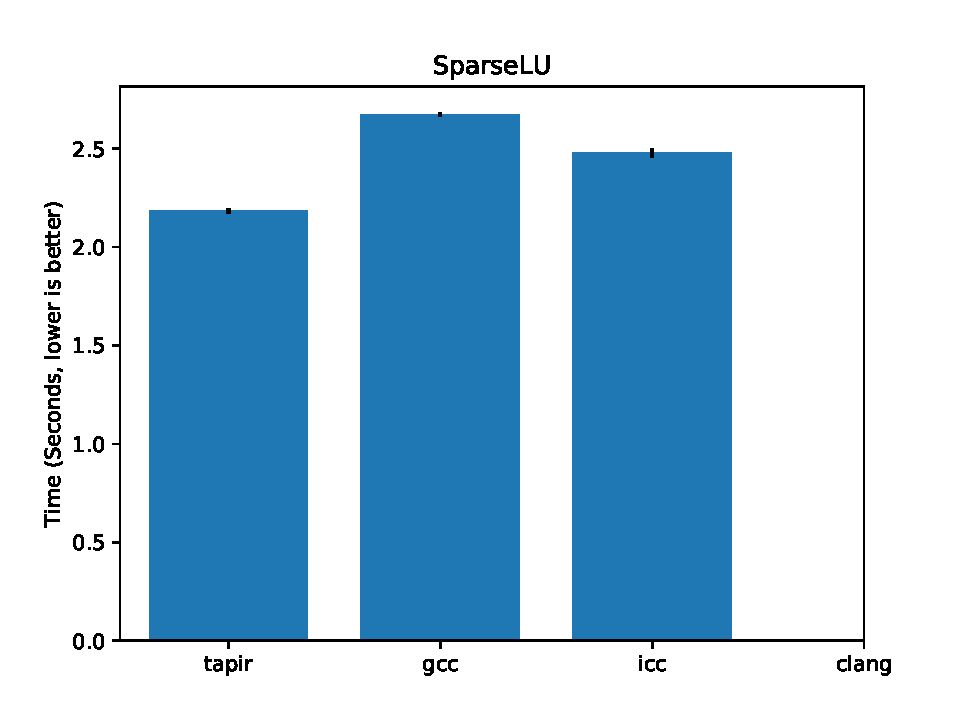
\includegraphics[width=\linewidth]{sparselu.pdf} 
\end{multicols}
\centering
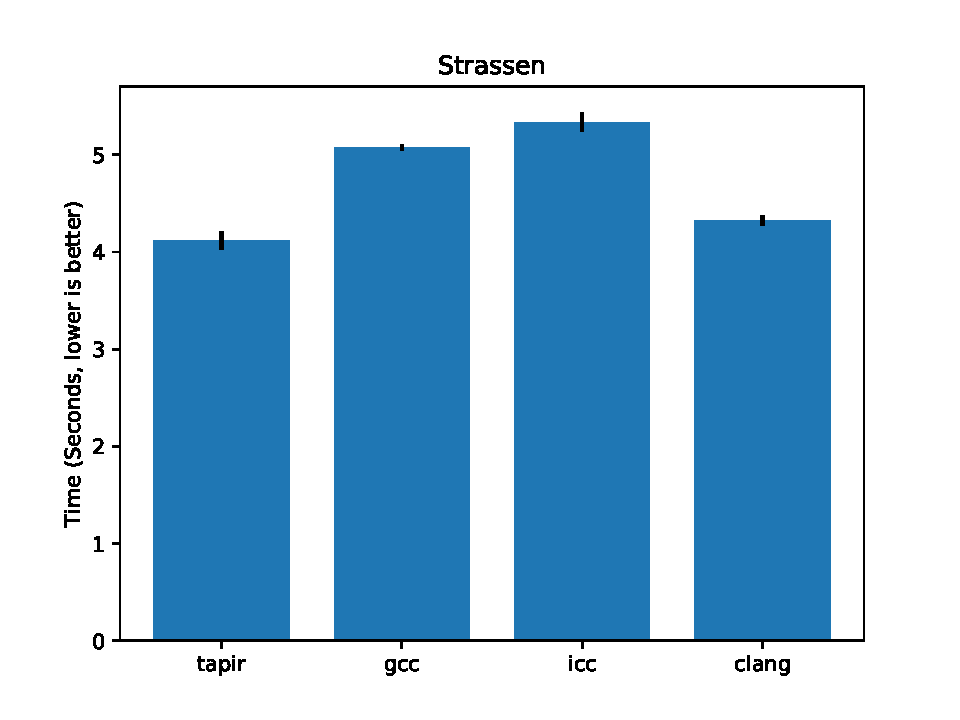
\includegraphics[width=0.45\linewidth]{strassen.pdf}
\caption{Barcelona OpenMP Task Suite Results (continued)}
\end{figure*}

The failure modes enumerated in Section~\ref{Sec:Evaluation} are denoted by 
asterisks in the implementation labels on the X axis. One asterisk refers to
some incorrect answers. Two asterisks refers to time-out. Three asterisks
refers to segmentation faults.

First, we can see that there is one failure for our implementation, on
\texttt{Floorplan}. Note that the result is non-zero. In fact, while ICC and
Clang finished in roughly 1-2 seconds, the our Tapir implementation was
finishing in \emph{0.02} seconds, and computing the correct result roughly half
the time. This raises interesting questions on the cost/benefit relation of the
OpenMP behaviour that our implementation is missing.

Other failures include ICC failing with segmentation faults on \texttt{FFT} and
\texttt{Fibonacci}. While we haven't carefully diagnosed these failures, we 
suspect that the number of tasks spawned exceeded a limit in Intel's compiler.
Note that the \texttt{FFT} failures were non-deterministic, occurring on
roughly one in three runs. Clang failed with segmentation faults on every run 
of \texttt{SparseLU}. Again, we didn't have the time to investigate these
failures, and are unsure what was causing them.

The final failures we saw were timeout failures. GCC was the only culprit for these
failures. Recall that the timeout was set at 10 minutes, so any timeout means GCC 
was running at least approximately 60 times slower than the fastest implementation. 
For example, on the \texttt{FFT} benchmark, while our Tapir implementation was running
in under 5 seconds, the GCC implementation was timing out at 600 seconds, so
was at least 100 times slower.

Putting failures aside for the moment, performance for our implementation is
quite strong, generally outperforming or matching the best of existing
implementations. For benchmarks where the overhead to work ratio is high is 
where the Tapir implementation really shines. For example, for the
\texttt{Fibonacci} benchmark, our implementation finishes significantly faster
than any of the others. While ICC failed for that sized input, we did test with
smaller inputs and found its similarly outpaced by the Tapir implementation.
\texttt{NQueens} and \texttt{FFT} show similar behaviour, to lesser degrees. In 
contrast, benchmarks that have a lower overhead to work ratio unsurprisingly 
differ less in performance. For example,  

\subsection{Forensics}

In this section we attempt to understand \emph{why} the performance varies in the ways 
it does. While we can't hope to figure out every discrepancy in performance, we
can hope to get some ideas for why the performance of our implementation is
generally better, and where each of the implementations is spending its time.

Our primary tool for this task will be performance counters. It's worth noting
that some information is difficult to infer from performance counters, such as
sources of contention in runtimes, reasons for memory locality issues, etc.
Still, it will give us some insight into performance bottlenecks in the
program.

Before we begin understanding why, it's worth noting again that the scope of the 
work that this paper is responsible for is only the frontend. All performance
gains due to the Cilk runtime we sadly cannot claim credit for.

Another import consideration is that we can break reasons for performance
discrepancies into a few categories: 

\begin{itemize}
\item Front-end code generation
\item IR Optimizations
\item Runtime efficiency
\end{itemize}

While we will try out best to distinguish between these in our forensics, it is 
difficult to do so with only performance counter information. A more thorough
investigation would require careful knowledge of each of the frontends and
runtimes. One thing we can guess at is that despite the focus of the paper,
\emph{IR optimisations are unlikely to be the cause of performance
improvements}. Our evidence for this comes from Shardl et al. \cite{}. While
some IR optimisations have been implemented, they seem to have significantly
more effect on parallel loop code , while the tasking code remains
relatively unaffected by IR optimizations \cite{}. 

\section{Discussion} \label{Sec:Discussion}

\subsection{Future Work} \label{Sec:Future}

\subsection{Related Work} \label{Sec:Related}

\section{Conclusion} \label{Sec:Conclusion}
We have shown that Tapir is an excellent IR target for OpenMP tasks. While not
all of the semantics are covered, we have a path forward for many of them. We have
shown that compiling to Tapir instructions allows for a straightforward compilation of 
OpenMP tasking programs to use the Cilk runtime system. We've also shown that this
combination leads to better performance than existing OpenMP tasking implementations
on the Barcelona OpenMP Tasking benchmark suite. Moving forward, we hope efforts like
this one help to reduce the fragmentation of parallel runtimes, as well as make
it easier to write optimization for parallel programs. 

\section*{Acknowledgment}
Sandia National Laboratories is a multimission laboratory managed and operated 
by National Technology and Engineering Solutions of Sandia, LLC., a wholly 
owned subsidiary of Honeywell International, Inc., for the U.S. Department of 
Energy’s National Nuclear Security Administration under contract DE-NA-0003525.

\bibliographystyle{ACM-Reference-Format}
\bibliography{annotated}

\end{document}
